\documentclass[10pt,a4paper,final]{article}
\usepackage[utf8]{inputenc}
\usepackage[portuguese]{babel}
\usepackage[T1]{fontenc}
\usepackage[margin=1in]{geometry}
\usepackage{amsmath}
\usepackage{amsfonts}
\usepackage[table]{xcolor}
\usepackage{graphicx}
\usepackage{multirow}
\usepackage{setspace}
\usepackage{amssymb}
\usepackage{lscape}
\usepackage{plano}
%\usepackage[alf]{abntex2cite}
\usepackage{natbib}
\usepackage{hyperref}
\usepackage{csquotes}

\programa{Engenharia Elétrica}
\area{Engenharia de Computação}
\aluno{Jefferson Carlos de Mendonça}
\orientador{Prof. Dr. Edson Satoshi Gomi}
\curso{Mestrado}
\dataIngresso{14/09/2016}
\titulo{Algoritmo para Categorização de Perguntas e Respostas do \textit{Site Stack Overflow}}
\resumo{Transformações no cenário tecnológico provocam mudanças constantes e exigem atualização contínua. Para manter-se atualizado, profissionais da área de computação recorrem à diversas fontes de informação, dentre elas destaca-se o site \textit{Stack Overflow}[1], maior comunidade de perguntas e respostas, onde os usuários podem aprender, trocar experiências e compartilhar conhecimento.
O objeto desta pesquisa é propor um algoritmo que consiga categorizar as perguntas e respostas deste \textit{website}. Uma vez que os questionamentos estejam devidamente indexados e organizados em tópicos, será possível detectar as dúvidas mais frequentes reportadas pelos usuários, permitindo que um assunto seja encontrado com maior facilidade, além de permitir que as entidades detentoras das tecnologias envolvidas usem os resultados obtidos para criar manuais e cursos que potencialize o entendimento da comunidade de interesse.}

\palavrachave{recuperação de informação}
\palavrachave{mineração de textos}
\palavrachave{classificação de textos}
\palavrachave{categorização automática de textos}
\palavrachave{extração de palavras chave}
\palavrachave{indexação de documentos}
\palavrachave{stack overflow}


\begin{document}

    \folhaDeRosto

    \plano
    
    \section{Introdução}
    
A evolução na área computacional se desenvolve em ritmo acelerado, algoritmos, técnicas para programação distribuída, testes automatizados, bancos de dados; todos estes assuntos têm algo em comum, a mudança frequente. As \emph{Linguagens de programação} seguem a mesma direção, suas API's - \textit{Application Programming Interface} são aprimoradas constantemente e muitas vezes incorporam novos paradigmas. Para acompanhar estas mudanças, profissionais da área de computação necessitam qualificação, que pode ser obtida através de cursos presenciais, a distância, livros, revistas, artigos e claro \textit{websites}.
\newline
\newline
 \cite{Manning2009} afirmam que a \textit{web} tornou-se a principal fonte por busca de informação e o relatório elaborado por \cite{Fallows} conclui que \enquote{ 92\% dos internautas dizem que a internet é um bom lugar para obter informações diariamente }.
Dentre estas fontes, merece destaque o fórum \textit{Stack Overflow} (SO), maior comunidade \textit{online} de perguntas e respostas onde os usuários podem aprender, trocar experiências e compartilhar conhecimento.
    
    \subsection{Contextualização do Problema}
O número de questões em sites de perguntas e respostas cresce diariamente, faz-se necessário categorizar os assuntos discutidos em tópicos, para uma busca mais eficiente e rápida. \cite{Manning2009} comparam este problema ao da procura de um livro em uma biblioteca, com certeza nossa busca será mais rápida e assertiva se os livros estiverem separados em prateleiras por assunto ou tópico. \cite{Yasotha2016} adicionam que a categorização manual de textos pode ser feita somente por especialistas e essa tarefa requer muito tempo. Como consequência é de grande importância a categorização e classificação de documentos de forma automática, ajudando os usuários a encontrarem informações relevantes para as suas necessidades.

    \subsection{Objetivos}
A proposta deste projeto de pequisa, é desenvolver um algoritmo que categorize e classifique os assuntos discutidos no SO.

    \subsection{Justificativas}

O método muito bem detalhado por \cite{Arash2016} categoriza os dados do SO. Em seu projeto os autores classificaram os assuntos utilizando as \textit{tags} da própria pergunta. No SO o próprio usuário, elege qual é a \textit{tag} da referida pergunta publicada. Apesar do grande avanço nesse campo de pesquisa, o uso de \textit{tags} limita a expansão da solução para outros fóruns que não possuem este recurso como, por exemplo, os \textit{sites} Quora[2] e Code Ranch[3].

   \subsection{Organização do texto}

Para melhor definir qual o posicionamento do presente projeto, no capítulo seguinte será detalhado em maior profundidade os projetos que abordaram a categorização de documentos, inclusive àqueles que também fizeram uso do site \textit{Stack Overflow} como base de dados. Então a proposta será detalhada quanto aos procedimentos para a indexação das perguntas e respostas, desde a seleção do conteúdo original, armazenamento em banco de dados e extração, por fim serão exibidos os resultados esperados. Segundo \cite{Kaleta2014} o termo indexação pode ser entendido como um dicionário de palavras-chave que representam o conteúdo de um texto.	

 \section{Revisão da Literatura}

A extração de informação do SO foi amplamente investigada por \cite{Arash2016}, uma vez que o site de interesse contém links para o Wikipédia[4], este foi escolhido como vocabulário controlado de palavras. Nesse projeto a análise de perguntas ficou limitada àquelas que possuem uma \textit{tag} que referencie uma palavra do vocabulário da base de conhecimento Wikipédia; em contra partida o ganho foi no mais de 4 milhões de artigos sobre os mais variados assuntos em todos os aspectos do conhecimento humano que esta base disponibiliza.
\newline
\newline
O processo adotado no trabalho anterior foi obter uma pergunta do SO, avaliar qual assunto ela representa através de suas \textit{tags} e então identificar qual a sua correspondente no Wikipédia. Com a informação identificada foi realizada a mineração de dados para detectar as categorias da referida pergunta. 
\newline
\newline
Apesar do enorme avanço, a pesquisa depende estritamente das \textit{tags} disponíveis e de um outro site, no caso o Wikipédia, para validar a palavra-chave encontrada e sua categoria. \cite{Mihalcea2004} propôs métodos para extração de sentenças e palavras-chave de um texto. O algoritmo é baseado em grafos que representam as interconexões das palavras que compõe o texto, essa abordagem requer certo volume de texto, quando testado em textos pequenos, como por exemplo, do tamanho de uma frase, a acurácia não foi a esperada para classificar o texto de uma pergunta.
 \newline
 \newline
Comparado com estes trabalhos, a investigação do SO será mais detalhada, será possível detectar o tópico de determinada pergunta sem informações extras além do texto, possibilitando a extensão da análise para outros fóruns de perguntas e resposta.
 

 \section{Detalhamento da Proposta}

Atualmente o SO possui cerca de 13 milhões de questões e pouco mais de 20 milhões de respostas[5], \cite{Krippendorff2012} sublinha que a mineração de texto vem sendo adotada como uma alternativa à situações em que a análise manual de grande quantidade dados se torna inviável. Análogo a metodologia proposta por \cite{Arash2016} a figura 1 exemplifica o processamento da informação desde sua obtenção até a produção dos resultados finais.
\newline
\newline
A primeira etapa é composta pela \textbf{coleta da informação}, o SO faz parte da rede de \textit{websites} StackExchange[6] que adota uma política de acesso livre à informação, ou seja, as postagens - perguntas e respostas, os usuários e os comentários são periodicamente disponibilizados de forma gratuita[7] para download e análise.
\newline
\newline
Na etapa de \textbf{extração da informação} será desenvolvido um algoritmo para extrair os assuntos principais \cite{Turney:2000:LAK:593957.593993} das dúvidas postadas no \textit{site}, assim como na proposta anterior também será utilizado o Wikipédia Miner \cite{Milne2012} como base de conhecimento sobre o vocabulário (palavras-chave) encontrado, de forma complementar também serão armazados a quantidade de vizualizações, a pontuação atribuída e o número de respostas da referida pergunta.
\newline
\newline
Por fim, na fase de \textbf{mineração do texto} será criado um \textit{ranking} \cite{mihalcea-tarau:2004:EMNLP} dos tópicos relevantes questionados com maior frequência, será utlizado o Gephi \cite{ICWSM09154} software \textit{open source} para exibir o grafo das categorias e suas interconexões.

\begin{figure}[!htb]
\centering
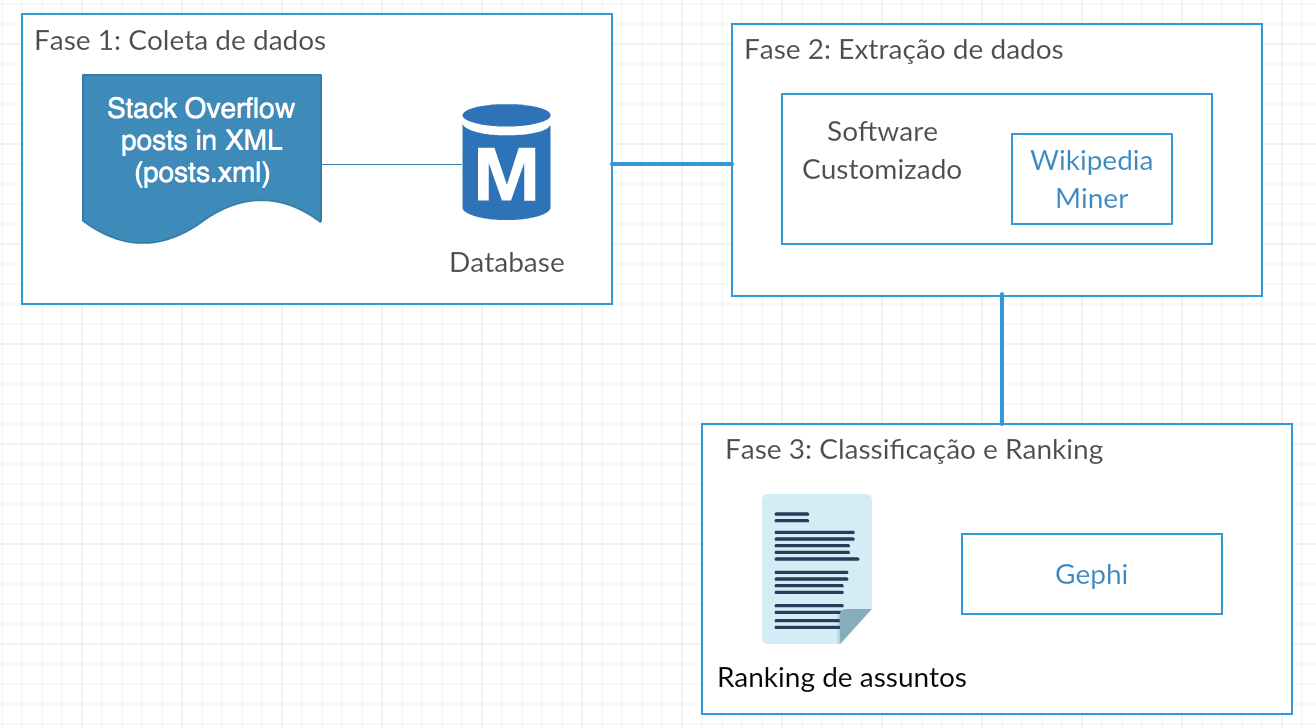
\includegraphics[height=8cm]{Figures/figura_1_metodologia}
\label{fig:figura_1_metodologia}   
\caption{Visão geral para categoriazação de perguntas e resposta do Stack Overflow.}
\end{figure}

  
    \section{Plano de Trabalho}

    \subsection{Resultados Desejados e Validação}
A análise será feita sobre o mesmo conjunto de dados da pesquisa realizada por \cite{Arash2016}, em seus trabalho \cite{Joorabchi2015} criaram exemplos de treinamento baseando-se nas ocorrências das \textit{tags} e nas categorias correspondentes identificadas no Wikipédia, os exemplos treinados utilizaram alguns algoritmos de aprendizagem de máquina, dentre eles: \textit{decision trees, bayes e support vector machines}. A acurácia obtida chegou à incríveis 98,8\%. É com base nesse cenário que a atual pesquisa pretende validar a extração automática de \textit{tags}, possibilitando a extensão da análise para outras fontes de dados.
 
    \subsection{Atividades e Cronograma}
    
Atividades:
    \begin{itemize}
    \item Disciplinas
	\item[] \quad Machine Learning
    \item[] \quad Metodologia Científica
    \item[] \quad Ciência de Dados
    \item[] \quad Inteligência Artificial
    \item[] \quad Fundamentos da Engenharia de Computação
    \item Revisão Literária
    \item Plano de Pesquisa
    \item Artigo Científico
    \item Projeto de Pesquisa
    \item[] \quad Fase 1: Coleta de dados
    \item[] \quad Fase 2: Extração de dados
    \item[] \quad Fase 3: Classificação e \textit{Ranking}
    \item Qualificação
    \item Defesa
    \end{itemize}

% ----------------------------------------------------------
% Cronograma
% ----------------------------------------------------------

\begin{figure}[!htb]
\centering
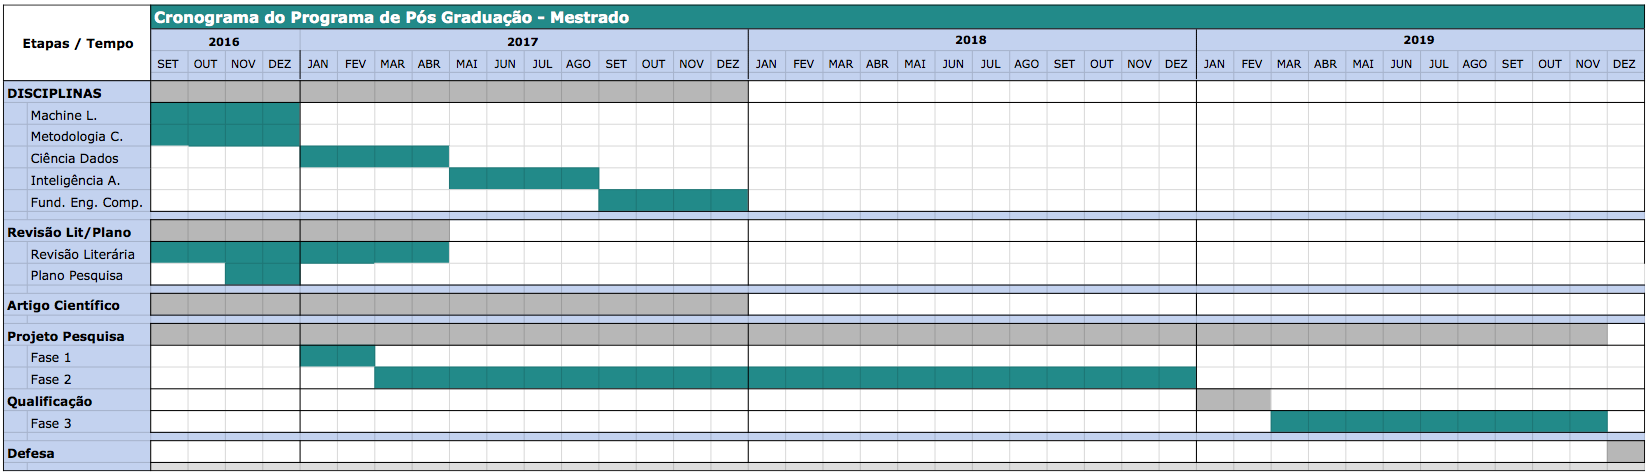
\includegraphics[height=4.8cm]{Figures/cronograma_projeto_project_timeline_retrato}\label{fig:cronograma_projeto_project_timeline_retrato}   
\caption{Cronograma.}
\end{figure}


% ----------------------------------------------------------
% Notas para links externos
% ----------------------------------------------------------

%%\chapter{Notes}
\textbf{\newline Notas}
\newline
\newline
1. http://stackoverflow.com/tour \newline
2. http://www.quora.com \newline
3. http://coderanch.com \newline
4. http://wikipedia.com \newline
5. http://data.stackexchange.com \newline
6. http://stackexchange.com \newline
7. https://archive.org/download/stackexchange

% ----------------------------------------------------------
% Referências bibliográficas
% ----------------------------------------------------------
\nocite{Joorabchi2015}
\nocite{Manning2009}
\nocite{Mihalcea2007}
\nocite{Mihalcea2001}
\nocite{Mihalcea2004}
\nocite{Milne}
\nocite{Miotto2013}
\nocite{Posch2014}
\nocite{Roul2015}
\nocite{Udell2005}
\bibliographystyle{apalike}
\bibliography{Refs}{}  


    

\end{document}
    